% Final Draft from arXiv.org -2024/05/19
\documentclass[journal]{IEEEtran}
%
%
\ifCLASSINFOpdf
  \usepackage[pdftex]{graphicx}
\else
  % DVI stuff 
\fi
%% For citation
\usepackage{cite}
% correct bad hyphenation here
\hyphenation{op-tical net-works semi-conduc-tor}


\begin{document}
%
\title{The Rise and Popularity of RISC-V}
%
\author{Saroj~Rout,~\IEEEmembership{Senior Member,~IEEE}\thanks{Dr. Saroj Rout is with Department of Electronics Engineering, Silicon Institute of Technology, Bhubaneswar, India (\texttt{https://sroutk.github.io}), email:\texttt{saroj.rout@silicon.ac.in}} and Chandra~Shekhar\thanks{Dr. Chandra Shekhar currently serves as the Professor Emeritus at Birla Institute of Technology \& Science, Pilani, Rajasthan, India} }

% The paper headers
\markboth{R\MakeLowercase{out \textit{et al.}}: The Rise and Popularity of RISC-V}{}

% make the title area
\maketitle

\begin{abstract}

RISC-V, a Reduced Instruction Set Computer (RISC) architecture has emerged as the architecture of choice for power-conscious devices such as tablets, mobile phones, and IoT embedded systems. This article looks at the evolution of RISC-V to give readers a historical perspective on its enormous success.  

\end{abstract}

% Note that keywords are not normally used for peerreview papers.
\begin{IEEEkeywords}
RISC-V, RISC, Computer Architecture
\end{IEEEkeywords}

%%%%%%%%%%%%%%%%%%%%%%%%%%%%%%%%%%%%%
% INTRODUCTION
%%%%%%%%%%%%%%%%%%%%%%%%%%%%%%%%%%%%%
\section{Introduction}

\IEEEPARstart{S}{ystems-on-a-chip} (SoC) with integrated processors are becoming ubiquitous. One such SoC is a microcontroller. It is hard to find an electronic system without a microcontroller in it, e.g. IoT, appliances, watches, toys, etc. They vary in complexity depending on the target applications. For example, Atmel's ATtiny series of microcontrollers are 8-bit processors starting with just 512-byte Flash and 32-byte SRAM running at 10 MHz clock speed \cite{microchip_attiny85_nodate}. On the other end of the spectrum are the popular STMicroelectronic STM32 series microcontrollers, which are based on Arm's Cortex-M 32-bit processor with up to 128 kB of L2 cache and more than 600 kB of SRAM running at 650 MHz \cite{stmicroelectronics_stm32_nodate}.

%%FIGURE : uC
\begin{figure}[htb]
    \centering
    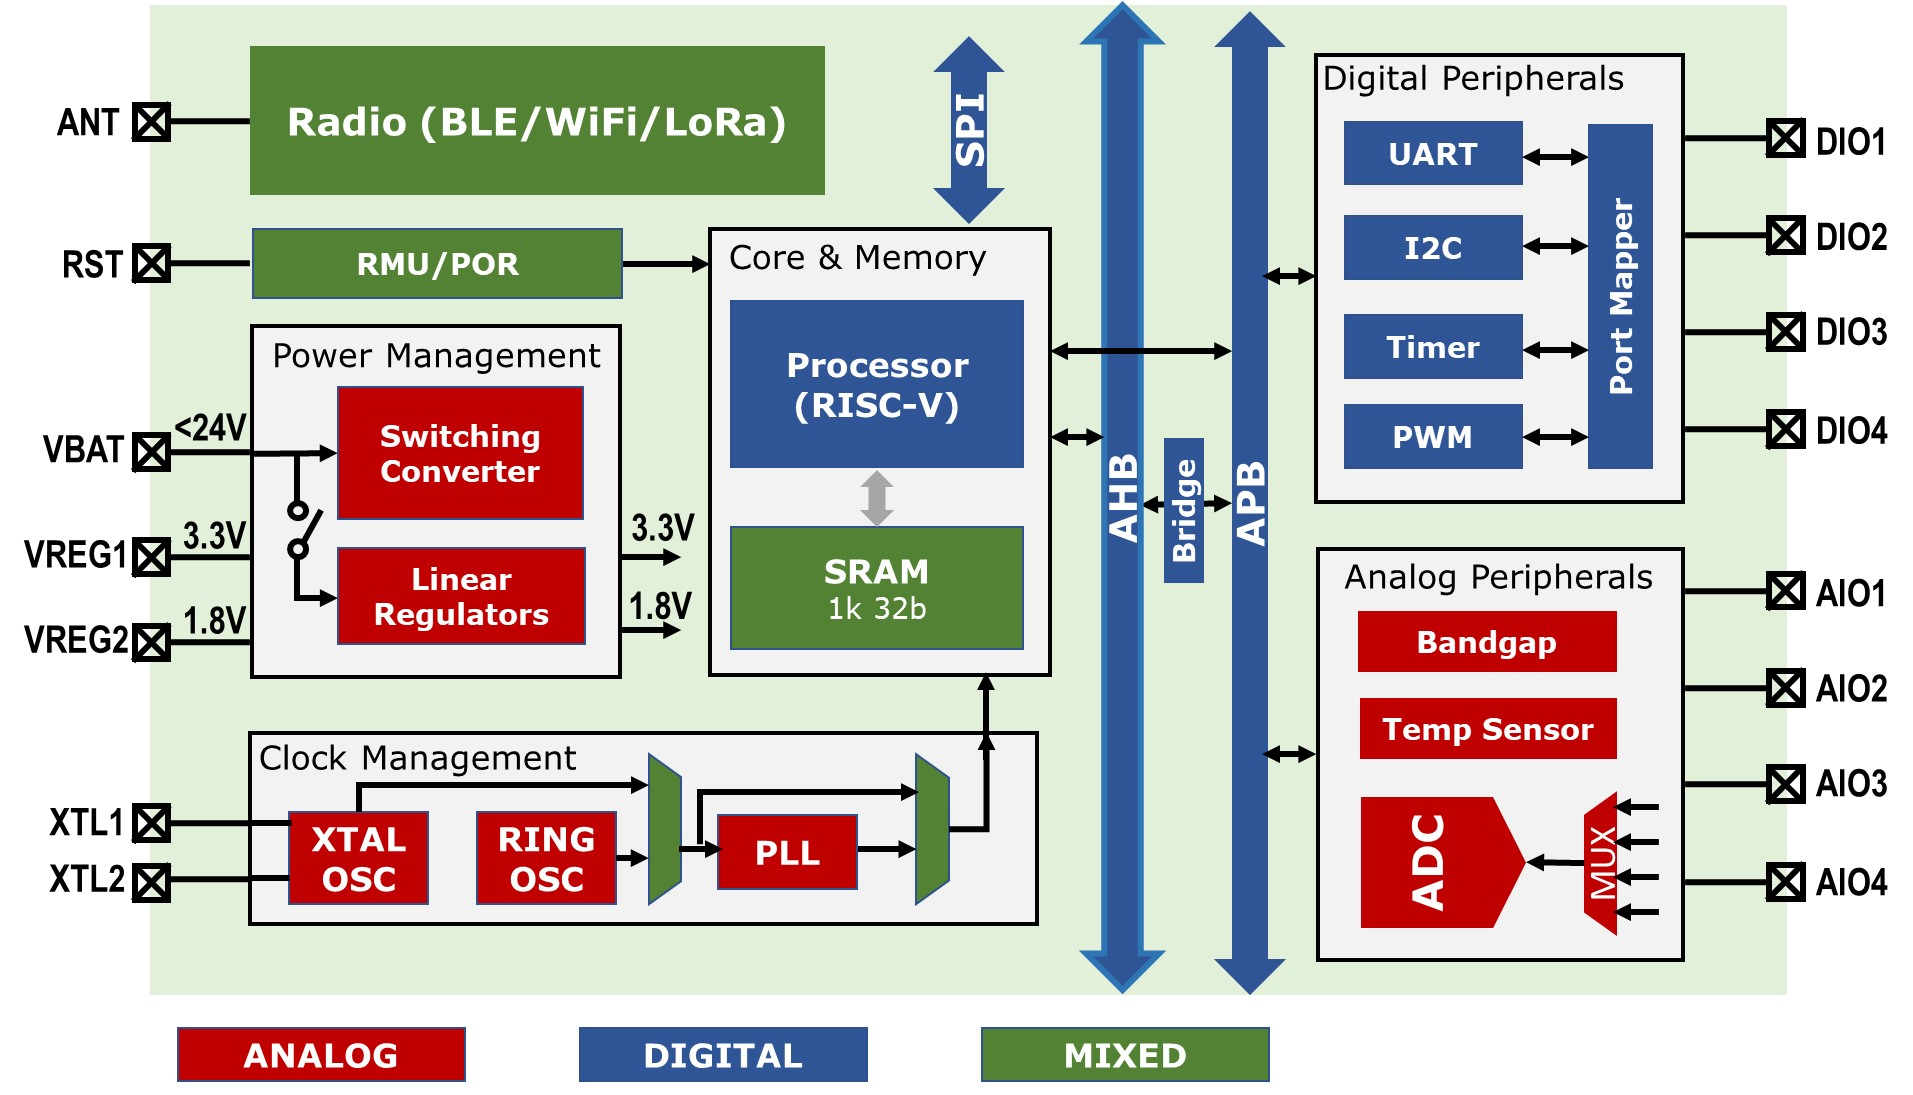
\includegraphics[width=0.95\linewidth]{image-uC.jpg}
    \caption{Architecture of a microcontroller intended for wireless IoT nodes.}
    \label{fig:uC}
\end{figure}

Fig.~\ref{fig:uC} shows an architecture of a microcontroller designed for wireless nodes of the Internet of Things (IoT). It contains a core processor, a cache (SRAM), analog peripherals (bandgap voltage reference, temperature sensor, and analog-to-digital converter(ADC)), digital peripherals (UART, SPI, PWM), power management, clock management (PLL, crystal oscillator) and RF Radio (Bluetooth, WiFi, LoRa \cite{sinha_survey_2017, bor_lora_2016}). Excluding the processor, all other components (often referred to as IPs) may be custom-designed by mixed-signal engineers or acquired through licensing from a supplier. The situation with respect to the processor is more complex. You can use a very old instruction set architecture (ISA) and implement it in your target technology. One such popular ISA is Intel's 8051 microcontroller architecture developed in 1980s \cite{noauthor_mcs-51_2023}. It has been around for several decades and has proven to be reliable, efficient, and versatile. Its compact size, low power consumption, and wide range of peripherals make it a popular choice for many embedded system applications. In addition, there is a large community of developers and engineers who are familiar with the 8051 architecture, making it easier to find support and resources for development. However, this architecture is appropriate for basic applications with minimal resource needs. For more complex applications, the 8051 architecture may be inadequate.

Companies like Arm, IBM, and Intel have very advanced and successful ISAs, but patents on key aspects of their ISAs prevent others from using them without licenses, which imposes a prohibitive cost for most educational, research organization or companies trying to target low-volume markets. 
Note that ISA is not an implementation of the hardware or software (OS, drivers, compilers). It is a standardization of the interface specification, so that development tools and design implementations can be reused and shared, provided that they are open and free. In addition, both hardware and software can be implemented in three ways: proprietary, licensed open-source, or free open-source.

There are three free and open-source RISC ISAs currently available for use\cite{asanovic_instruction_2014}:
\begin{enumerate}
    \item \emph{SPARC V8} from Sun Microsystems that was made into a IEEE standard in 1994.
    \item \emph{OpenRISC} is a GNU open-source effort started in 2000, with 64-bit ISA completed in 2011.
    \item \emph{RISC-V} (pronounced "RISC 5") is a BSD-licensed open source project initiated in 2010 at the University of California, Berkeley by Krste Asanovic, David A. Patterson and their graduate students Andrew Waterman and Yunsup Lee, influenced in part by the intellectual property limitations of ARM and the absence of 64-bit addressing and the complexity of ARM v7.
\end{enumerate}

Before we look at the history of RISC-V and why it prospered compared to it's predecessors SPARC V8 and OpenRISC, it is worth taking a quick look at the history of microprocessors and how RISC has emerged as the goto architecture for power-conscious devices such as tablets, mobile phones, and embedded systems.

%%%%%%%%%%%%%%%%%%%%%%%%%%%%%%%%%%%%%
% BRIEF HISTORY OF MICROPROCESSORS
%%%%%%%%%%%%%%%%%%%%%%%%%%%%%%%%%%%%%
\section{Brief History of Microprocessors}

The birth of a microprocessor took place around the end of 1960s when a Japanese calculator maker Business Computer Corporation (Busicom) contracted with Intel, then a small startup, for custom chips for a calculator. That gave birth to Intel 4004 which is widely accepted as the first microprocessor, and that calculator was launched in early 1971 with Intel 4004 in it along with chips for storage and I/O \cite{faggin_history_1996}. In early 1970, Computer Terminal Corporation (CTC), a company based in San Antonio, TX, USA, arranged Intel to build a single MOS chip to replace their discrete-based 8-bit processor for their general-purpose computer, Data Point 2200. Although Intel went ahead and built the chip based on the Data Point 2200 architecture, the project was suspended as CTC contracted Texas Instruments (TI) for the job \footnote{An interesting historical note: Intel was a startup with about 100 employees, and Texas Instruments was a large company with more than 45,000 employees}. TI developed the TMC 1795 processor for CTC which was rejected after testing the chip. Eventually, TI discontinued the project due to unsuccessful attempts to sell it to other companies. In the mean time, Intel 8008 was successfully working at the end of 1971, but CTC had lost interest in that project and gave up its exclusive right to design. Intel then commercialized 8008 in April 1972, and went on to become a successful product. In 1974, the development of the 8008 led to the creation of the Intel 8080. This processor significantly shaped the Intel 8086 and modern x86 architecture, which became predominant in the personal computer (PC) and server industries \cite{noauthor_intel_2024}. Thus, the historical narrative is indeed fascinating, beginning with CTC's Data Point 2200 computer, which ultimately positioned Intel as a key player in the microprocessor industry and its x86 architecture as a dominant force in subsequent years.

From 1978 until 1988, the architecture of the complex instruction set computer (CISC) dominated the market \cite{blem_power_2013}, with a performance improvement of averaging 15\% per year. This improvement mainly owed to Moore's law, which ensured the doubling of transistors per unit area every 18 months, and Dennard's scaling theory to ensure that the power consumed in the chip also remained about the same.

From 1988-2003, the focus shifted to improving single-processor performance by exploiting instruction level parallelism (ILP), which led to Reduced Instruction Set Computer (RISC) architecture becoming mainstream \cite{patterson_risc_1998}. Single processor performance improved tremendously with the use of pipelining for single-cylce execution, branch prediction, out-of-order execution, on-chip caches, multilevel on-chip caches, superscalar processors, and VLIW. The continuing benefit of Moore's law and the improvement in Dennard scaling performance were averaged at 40\% per year.
This performance enhancement was the result of the change in the RISC Instruction Set Architecture (ISA) and microarchitectures based on pipelined execution. RISC offered a simplified ISA that restricted arithmetic and logic operations to register operands as source and destination operands. Memory access was limited to two instructions, load and store, without performing any logic or arithmetic operation on the operands. Memory addressing modes were fewer and simpler compared to CISC. The RISC ISA also allowed for ILP through pipelining of instructions that gives a throughput of one instruction per cycle, in contrast to a CISC architecture taking multiple cycles for an instruction to execute. Furthermore, the RISC ISA enabled superscalar processing, permitting multiple instructions to enter the pipeline simultaneously, though this process faced certain difficulties. 

Following over ten years of leveraging Moore's law and Dennard's scaling, the computer architecture field was compelled to seek innovative ways to enhance performance annually. In this progressive journey, the RISC architecture gradually became the preferred choice.
 
%%%%%%%%%%%%%%%%%%%%%%%%%%%%%%%%%%%%%
% The Emergence of RISC-V as Free, Open ISA 
%%%%%%%%%%%%%%%%%%%%%%%%%%%%%%%%%%%%%
\section{The Emergence of RISC-V as Free, Open ISA }
For an open-source ISA to have a long and successful lifespan, the founders of RISC-V were wise to look for a proven commercial record. This quickly eliminated some unsuccessful ones or those that have slowly died down, including the \textit{ stack} ISA, \textit{VLIW}, Multiflow, and any new CISC ISAs. While 80x86 had dominated the PC market, \textit{RISC-style} load-store ISAs date back to Seymour Cray's CDC 6600 and RISC had dominated the mobile and tablets of the post-PC Era. Therefore, RISC naturally emerged as a free, open ISA. The founders and the community also felt the need to start with a clean slate with a new RISC ISA to correct some of the mistakes of its predecessors. Some of the learning from the mistakes were: \textit{leaving out essentials} such as the byte load / store or the half word load / store in the initial MIPS I, \textit{making the ISA bulky} by including too much like the register windows in SPARC, or \textit{microarchitectural dependent ISA} like the delayed branch in MIPS. 

Given that the longevity of ISA is in decades, it was essential to look at the future technology landscape to predict some essential features of this new ISA. Three technology platforms seemed to dominate: Internet of Things (IoT), Personal Mobile Devices, and Warehouse-Scale Computers (WSCs). To target these technologies, it will be essential to have four key features from the new ISA:
\begin{itemize}
    \item \textit{Base-plus-extension ISA} with a small core set of instructions for cost-sensitive applications, optional extensions with standard ISA additions to customize SoCs, and space for entirely new set of instructions application-specific SoCs.
    \item \textit{Compact instruction set encoding} for cost-sensitive applications such as IoT that require smaller memory.
    \item \textit{Quadruple-precision (QP) as well as SP and DP} support for wide-ranging data size requirements from WSCs to IoT.
    \item \textit{128-bit addressing} as well as \textit{32-bit and 64-bit}.
\end{itemize}

%%FIGURE : Free ISA score table
\begin{figure}[htb]
    \centering
    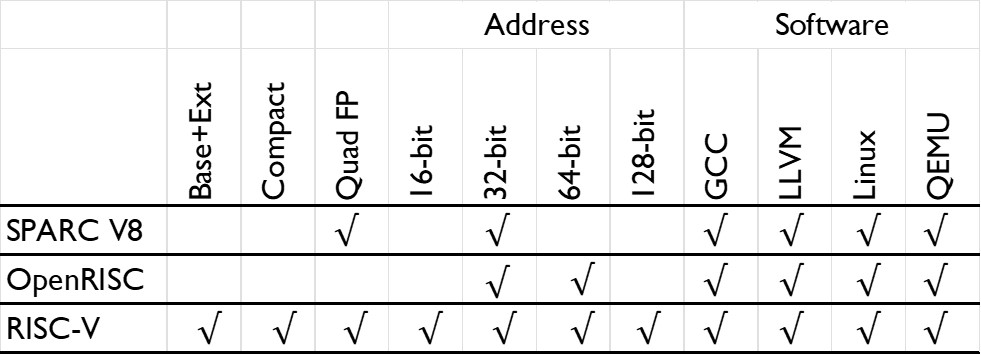
\includegraphics[width=0.95\linewidth]{image-3FreeISA-Table.jpg}
    \caption{Scores for three free open ISAs using four criteria plus listing critical compilers and OS ports.}
    \label{fig:score}
\end{figure}

Fig.\ref{fig:score} tabulates the scores of the three free ISAs based on four criteria plus the list of critical compilers and OS ports. RISC-V meets all the intended requirements while being simple and clean. Due to these benefits, RISC-V quickly became popular within the community and emerged as the preferred option for a free and open-source ISA. In particular, Chisel \cite{bachrach_chisel_2012} from Berkeley is a highly productive open hardware design system that became part of many silicon successes, making the case for RISC-V even stronger. 
RISC-V continues to evolve, with the ratification of new specifications, including RISC-V profiles, Volume II cryptography extensions, and the Input-Output Memory Management Unit (IOMMU) architecture specification \cite{mcmahon_risc-v_nodate}.
%https://riscv.org/announcements/2021/12/risc-v-celebrates-incredible-year-of-growth-and-progress-ratifying-multiple-technical-specifications-launching-new-education-programs-and-accelerating-broad-industry-adoption/
A notable advancement is the introduction of a 16-bit compressed instruction set, C \cite{waterman_risc-v_2015}, which reduces the code size by approximately 50 to 60\% in RISC-V programs. This extension uses a concise 16-bit format for common operations, compatible with all base ISAs (RV32, RV64, RV128) and other standard instruction extensions.

The rise and popularity led to the RISC-V Foundation (www.riscv.org), a nonprofit corporation that was founded in 2015 to build an open and collaborative community of software and hardware innovators based on the RISC-V ISA. In November 2018, the RISC-V Foundation announced a joint collaboration with the Linux Foundation to provide operational, technical, and strategic support.

%%%%%%%%%%%%%%%%%%%%%%%%%%%%%%%%%%%%%
% Latest Advances in RISC-V Technology
%%%%%%%%%%%%%%%%%%%%%%%%%%%%%%%%%%%%%
\section{Latest Advances in RISC-V Technology}
RISC-V has gained widespread commercial acceptance in multiple sectors, including automotive embedded systems, large-scale artificial intelligence, 5G technologies, and high-performance computing. This section presents several prominent examples.

Intel's announcement of a \$1 billion fund to support RISC-V chip development highlights its increasing significance. RISC-V chips are now being used in devices such as earbuds, hard drives, and AI processors, with over 10 billion cores shipped. Companies are also considering RISC-V for data centers and spacecraft \cite{chen_chip_nodate}.
The adoption of RISC-V cores in different industries is predicted to reach 62 billion cores by 2025. A study in 2020 showed almost a quarter of ASIC and FPGA projects incorporating RISC-V cores \cite{redmond_risc-v_2021} and recent trends support this assertion.
Imagination Technologies' RISC-V APXM-6200 CPU, a 64-bit in-order processor with an 11-stage pipeline, is designed for consumer and industrial applications. It offers a high performance density, outperforming the Arm Cortex-A510 in integer performance at similar clock speeds. The inclusion of an SDK with AI libraries, a Visual Studio Code extension, and TEE certification partnerships underscores the increasing adoption of RISC-V in the industry \cite{krewell_imagination_2024}.
The Titanium Ti375 FPGA by Efinix integrates a quad-core RISC-V, 370,000 logic elements, and features including a Linux-capable MMU, FPU, and custom instructions, making it ideal for AI and edge computing. It also contains a dual transceiver, LPDDR4 DRAM controller, and MIPI D-PHY, all manufactured with 16 nm technology \cite{nordyk_fpga_2024}.
The Roma laptop, the first designed for RISC-V development, features a quad-core 1.5GHz 64-bit CPU, a dual-core GPU, 8GB RAM, 128GB eMMC storage, and a 1TB SSD. It runs on the multilingual openKylin OS, aimed at helping developers create RISC-V software, indicating a significant advancement in the RISC-V ecosystem \cite{ouz_worlds_nodate}.
The R9A02G021 MCU, equipped with a 32-bit Renesas RISC-V core, 4 kB of data flash and 16 kB of ECC SRAM, is optimized for energy efficiency and performance. It includes extensive analog features, multiple timers, various serial interfaces, and regulated IOs. Renesas provides a robust ecosystem to support development, highlighting the role of the RISC-V architecture in enhancing design flexibility across industries \cite{noauthor_ultra-low_nodate}.

%%Conclusion
\section{Conclusion}
The history thus far has clearly indicated in favor of RISC-V as a free and open ISA. It has created a great opportunity by removing barriers related to design risk, cost of entry, partner limitations, and supply chain. The RISC community took a united approach to learn from previous mistakes of open ISAs and created an ISA for longevity. Given the increasing success of RISC-V, it can be safely envisioned to be the choice of ISA for most power-conscious and those with costs, including IoT, WSC, and mobile devices.  

%%Bibliography
\bibliographystyle{IEEEtran}
\bibliography{SRout-RISCV-main}

\end{document}

